\documentclass{beamer}
\setbeamertemplate{section in toc}[sections numbered]
\usefonttheme[onlymath]{serif}
\beamertemplatenavigationsymbolsempty
\setbeamertemplate{footline}{% 
  \hfill% 
  \usebeamercolor[gray!50]{page number in head/foot}% 
  \usebeamerfont{page number in head/foot}% 
  \insertframenumber\,/\,\inserttotalframenumber%
}
\usepackage{amsmath}
\usepackage{graphicx}
\usepackage[tight,FIGTOPCAP]{subfigure}
\usepackage{lmodern}
\usepackage{amsmath}
\usepackage{braket}
\usepackage{color}
\usepackage{bm}
\usepackage{amssymb}
\usepackage{bbold}
\usepackage{tikz}
\usepackage{tikz-cd}
\usepackage{empheq}
\usepackage{caption}
\usepackage{stackengine}
\usepackage{framed}
\usepackage[percent]{overpic}
\usepackage{adjustbox}
\DeclareMathOperator{\sgn}{sgn}
\tikzset{>=latex}
\usetikzlibrary{matrix,calc,arrows,patterns,angles,quotes,shapes.geometric,positioning,decorations.pathreplacing,decorations.markings}
\newcommand{\blue}[1]{{\color{blue}{#1}}}
\newcommand{\ms}{\mathsf}
\renewcommand{\(}{\left(}
\renewcommand{\)}{\right)}
\renewcommand{\[}{\left[}
\renewcommand{\]}{\right]}
\tikzset{
  % style to apply some styles to each segment of a path
  on each segment/.style={
    decorate,
    decoration={
      show path construction,
      moveto code={},
      lineto code={
        \path [#1]
        (\tikzinputsegmentfirst) -- (\tikzinputsegmentlast);
      },
      curveto code={
        \path [#1] (\tikzinputsegmentfirst)
        .. controls
        (\tikzinputsegmentsupporta) and (\tikzinputsegmentsupportb)
        ..
        (\tikzinputsegmentlast);
      },
      closepath code={
        \path [#1]
        (\tikzinputsegmentfirst) -- (\tikzinputsegmentlast);
      },
    },
  },
  % style to add an arrow in the middle of a path
  mid arrow/.style={postaction={decorate,decoration={
        markings,
        mark=at position .5 with {\arrow[#1]{stealth}}
      }}},
}

%Information to be included in the title page:
\title{Chiral Dirac Superconductors: Second-order and Boundary-obstructed Topology}
%\author{Apoorv Tiwar, Ammar Jahin, and Yuxuan Wang}
%\institute{University of Florida}
\date{University of Florida, May 2020}

\begin{document}
\frame{\titlepage 
    } 

\begin{frame}
    \centering
    \begin{columns}
        \begin{column}{0.5\textwidth}
            \centering
            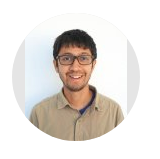
\includegraphics[trim= 0 20 0 20,clip]{Screenshot_20200516_213116.png}

            Apoorv Tiwari
            
            University of Zurich
        \end{column}
        \begin{column}{0.5\textwidth}
            \centering
            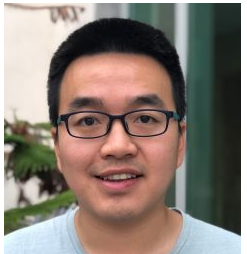
\includegraphics[scale=0.4]{YWSC.png}

            Yuxuan Wang 

            University of Florida
        \end{column}
    \end{columns}
\end{frame}

\begin{frame}
    \frametitle{Introduction}
    \begin{itemize}
        \item The problem we study is that of a 2D Dirac semi-metal with $p+ip$ paring in the superconducting state. 
        \item We ask what kind of topology can be found in such systems. \pause 
    \end{itemize}
    \vspace{0.4cm}
    Quick answer (the goal of this talk is to explain this quick answer): 
    \begin{columns}
        \begin{column}{0.5\textwidth}
                \begin{table}
                    \centering
                    \def\arraystretch{0.4}
                    \begin{adjustbox}{width=\columnwidth,center}
                        \begin{tabular}{|| p{2.5cm}| p{2.5cm} | p{2.5cm}||} 
                        \hline
                        \begin{center} Model \end{center} 
                        &  \begin{center} With $C_{4}$ \end{center}   & \begin{center} With $C_{2}$  \end{center} \\ 
                        \hline\hline
                        \begin{center}
                        With PH
                        \end{center}
                        & %\rule{0pt}{4.6ex}
                        \begin{center}
                        HOTSC$_{2}$; \\
                        %\newline with 
                        corner Majorana 
                        %{\rule[-3.2ex]{0pt}{0pt}} 
                        \end{center}
                        & 
                        \begin{center}
                        BOTSC$_2$; \\
                        %\newline with 
                        corner Majorana 
                        \end{center}
                        \\ 
                        \hline
                        \begin{center}
                        Without PH
                        \end{center} &
                        \begin{center}
                        HOTI$_{2}$; \\
                        %\rule{0pt}{4.6ex}
                        % \newline with 
                        filling anomaly
                        % {\rule[-3.2ex]{0pt}{0pt}}
                        \end{center}
                        & 
                        \begin{center}
                        Trivial
                        \end{center}
                            \\ 
                        \hline
                        \end{tabular}
                \end{adjustbox}
            \end{table}
        \end{column}
        \begin{column}{0.5\textwidth}
            HOTI = Higher Order Topological Insulator

            HOTSC = Higher Order Topological Superconductor

            BOTSC = Boundary Obstructed Topological Superconductor
        \end{column}
    \end{columns}

\end{frame}

\begin{frame}
    \frametitle{Outline}
    \tableofcontents
\end{frame}

\AtBeginSection[]
{
\begin{frame}
    \frametitle{Outline}
    \tableofcontents[currentsection]
\end{frame}
}

\section{The model}
\subsection{Dirac + \texorpdfstring{($p+ip$)}{}}

\begin{frame}
    \frametitle{The normal state}
    \begin{columns}
    \begin{column}{0.8\textwidth}
        We take 4 Dirac points in the normal state as a given. 
        In general a Dirac semi-metal in 2D can be modeled by, 
        \begin{align*}
            \mathcal{H}^{\text{normal}}(\bm k) = f_1(\bm k) \sigma_x + f_2(\bm k) \sigma_z -\mu 
        \end{align*}
    \end{column}
    \begin{column}{0.2\textwidth}
        \begin{figure}[t]
            \centering
            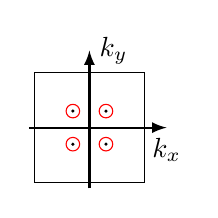
\begin{tikzpicture}[scale=0.7]
                \draw (-1,-1) -- (1,-1) -- (1,1) -- (-1,1) -- cycle;
                \draw[thick,->] (-1.1,0) -- (1.4,0) node[anchor=north] {$k_x$};
                \draw[thick,->] (0,-1.1) -- (0,1.4) node[anchor=west] {$k_y$};
                \draw[fill=black] (0.3, 0.3) circle (0.5pt);
                \draw[fill=black] (-0.3, 0.3) circle (0.5pt);
                \draw[fill=black] (0.3, -0.3) circle (0.5pt);
                \draw[fill=black] (-0.3, -0.3) circle (0.5pt);
                \draw[red] (0.3, 0.3) circle (3.5pt);
                \draw[red] (-0.3, 0.3) circle (3.5pt);
                \draw[red] (0.3, -0.3) circle (3.5pt);
                \draw[red] (-0.3, -0.3) circle (3.5pt);
            \end{tikzpicture}
            

        \end{figure}
        
    \end{column}
    \end{columns}\pause

    \vspace{0.5cm}
    The Dirac points can be protected by a chiral symmetry or a product of time-reversal and inversion, but neither of these two symmetries will be preserved in the superconducting state. \pause
    \begin{columns}[b]
    \begin{column}{0.35\textwidth}
        \centering
        \begin{align*}
            &\hat{C}_4 = \frac{1}{\sqrt{2}} (\sigma_x + \sigma_z) \\ 
            &\hat{C}_2 = \hat{C}_4^2 = \mathbb{1} 
        \end{align*} 
    \end{column}
    \begin{column}{0.65\textwidth}
        \begin{minipage}[b][0.2\textheight][c]{\linewidth}
            \vspace{0.8cm}
            \begin{empheq}[box=\fbox]{align*}
                \hat{C}_{4} (\sigma_z,\sigma_x) \hat{C}^{-1}_{4} =  (\sigma_x,\sigma_z)
            \end{empheq}
            \begin{align*}
                \hat{C}_{4/2} \mathcal{H}^{\text{normal}}(\bm k) \hat{C}^{-1}_{4/2} =  \mathcal{H}^{\text{normal}}(C_{4/2} \bm k)
            \end{align*} 
        \end{minipage}
    \end{column}
    \end{columns}\pause
    \vspace{0.3cm}
    \begin{empheq}[box=\fbox]{align*}
        f_1(\bm k) = f_1(-\bm k) \text{,\ and\ } f_2(\bm k) = f_2(-\bm k)
    \end{empheq}

\end{frame}

\begin{frame}
    \frametitle{Adding pairing terms}
    Adding a finite range attractive potential between the electrons gives a leading instability of the system toward a $p + ip$ pairing. \pause
    The superconducting BdG Hamiltonian: 
    \begin{columns}
    \begin{column}{0.67\textwidth}
        \begin{align*}
            \mathcal{H}(\bm k) &= f_1(\bm k) \sigma_x \tau_z + f_2(\bm k) \sigma_z \tau_z \\
            &+ \Delta g_1(\bm k)  \tau_x + \Delta g_2(\bm k) \tau_y -\mu \tau_z,
        \end{align*} 
    \end{column}
    \begin{column}{0.33\textwidth}
        where $\tau_i$ act on the Nambu space. 
    \end{column}
    \end{columns}\pause
    \begin{align*}
        \mathcal{P} \mathcal{H}(\bm k) \mathcal{P}^{-1} = - \mathcal{H}(-\bm k),  && \mathcal{P} = \tau_x K
    \end{align*}
    \begin{empheq}[box=\fbox]{align*}
        g_1(\bm k) = -g_1(-\bm k) \text{,\ and\ } g_2(\bm k) = -g_2(-\bm k)
    \end{empheq}\pause

    For $\mu=0$ the model has a chiral symmetry, 
    \begin{align*}
        \mathsf{S} \mathcal{H}(\bm k) \mathsf{S}^{-1} = -\mathcal{H}(\bm k), && \mathsf{S} = \sigma_y \tau_z
    \end{align*}
\end{frame}

\begin{frame}
    \frametitle{$C_4$ and $C_2$ symmetries for the BdG Hamiltonian}
    \begin{columns}
    \begin{column}{0.5\textwidth}
        \begin{align*}
            &\hat{C}_4 = \frac{1}{\sqrt{2}} (\sigma_x + \sigma_z) e^{\frac{i\pi}{4}\tau_z} \\
            &\hat{C}_2 = \hat C_4^2 = e^{\frac{i2\pi}{4}\tau_z} \\
            &\hat{C}_4^4 = \hat C_2^2 =  - \mathbb{1}.
        \end{align*}
    \end{column}
    \begin{column}{0.5\textwidth}
        For the $C_{4/2}$ symmetric case: 
        \begin{align*}
            \hat{C}_{4/2} \mathcal{H}(\bm k) \hat{C}^{-1}_{4/2} = \mathcal{H}(C_{4/2} \bm k)
        \end{align*}
    \end{column}
    \end{columns}\pause 
    \begin{columns}
        \begin{column}{0.45\textwidth}
            A prototypical example: 
            \begin{align*}
                \mathcal{H}(\bm k) &= (\gamma_x + \cos(k_x)) \sigma_x \tau_z \\ 
                & + (\gamma_y + \cos(k_y))\sigma_z \tau_z \\
                & +\Delta \sin(k_x) \tau_x \\
                &+ \Delta \sin(k_y) \sigma_x \tau_y -\mu \tau_z,
            \end{align*} 
        \end{column}
        \begin{column}{0.55\textwidth}
            \begin{figure}[]
                \centering
                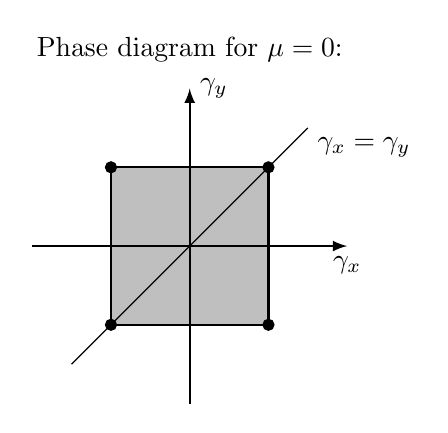
\begin{tikzpicture}
                    \node[align=center] at (0,2.5) {Phase diagram for $\mu=0$:};
                    \draw[fill=gray!50,draw=black, thick] (-1,-1) rectangle (1,1);
                    \draw[black] (-1.5,-1.5) -- (1.5,1.5) node[anchor=north west] {$\gamma_x = \gamma_y$};
                    \draw[fill, black] (-1,-1) circle (2pt) (1,-1) circle (2pt) (-1,1) circle (2pt) (1,1) circle (2pt);
                    \draw[thick,->] (-2,0) -- (2,0) node[anchor=north] {$\gamma_x$};
                \draw[thick,->] (0,-2) -- (0,2) node[anchor=west] {$\gamma_y$};
                \end{tikzpicture}
            \end{figure}
        \end{column}
    \end{columns}
\end{frame}


\begin{frame}
    \frametitle{Edge spectrum and Majorana zero modes}
    For $\gamma_x = \gamma_y = 0.5$, $\Delta = 0.4$, and $\mu = 0.2$.
    \begin{figure}[]
        \centering
        \stackunder[0pt]{On a cylindrical:}{
        \subfigure{
        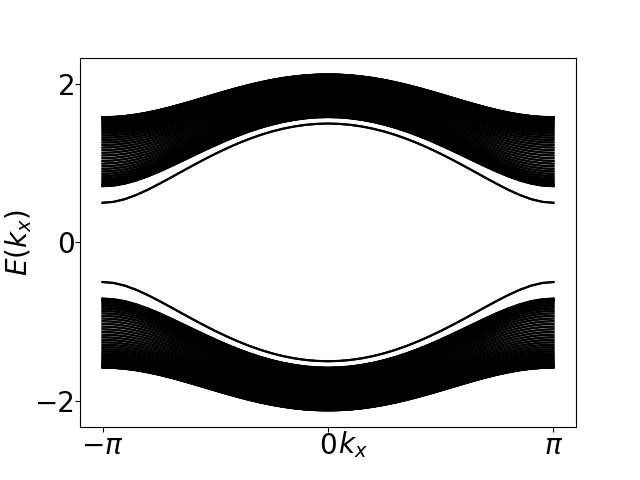
\includegraphics[trim=0 15 0 35,clip, scale=0.3]{energy_cylinder.png}%
        }}\pause
        \stackunder[0pt]{With open boundaries:
        }{\subfigure{
            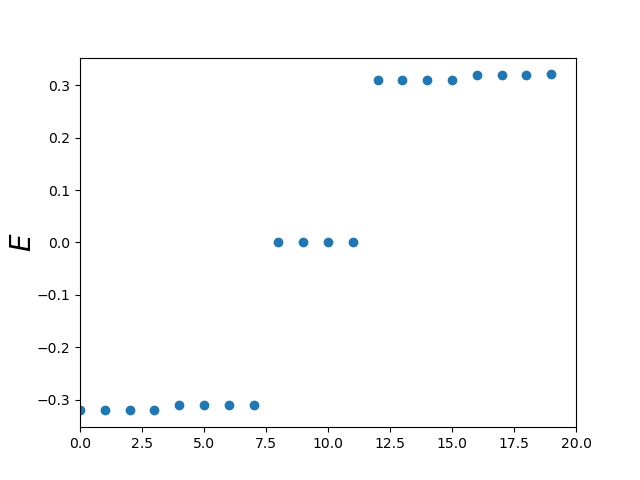
\includegraphics[trim=0 22 0 42,clip, scale=0.3]{energy_open_majorana_zero.png}%
        }}\pause

        \stackunder[0pt]{Zero modes:}{\subfigure{
            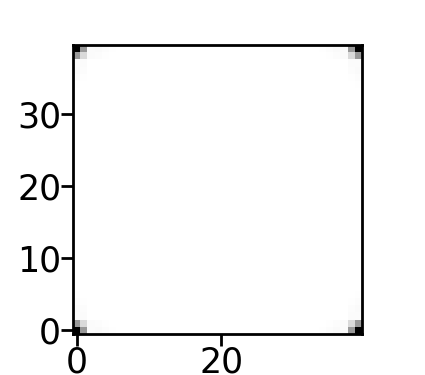
\includegraphics[trim=0 0 0 13,clip,scale=0.9]{corner_modes_2.png}%
        }}\pause
        \qquad \qquad
        \subfigure{
            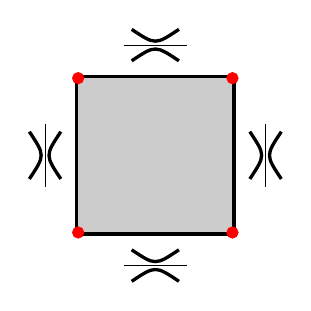
\begin{tikzpicture}[scale=1.0]
                \draw[] (-0.4,1.4) -- (0.4,1.4);
                \draw[very thick] (-0.3, 1.6) .. controls (0,1.4) .. (0.3,1.6);
                \draw[very thick] (-0.3, 1.2) .. controls (0,1.4) .. (0.3,1.2);
    
                \draw[] (1.4,-0.4) -- (1.4,0.4);
                \draw[very thick] (1.6, -0.3) .. controls (1.4,0) .. (1.6,0.3);
                \draw[very thick] (1.2, -0.3) .. controls (1.4,0) .. (1.2,0.3);
    
                \draw[fill=black!20!white, draw=black, very thick] (-1,-1) rectangle (1,1);
                \draw[fill, red] (0.98,0.98) circle (2pt) (-0.98,0.98) circle (2pt) (0.98,-0.98) circle (2pt) (-0.98,-0.98) circle (2pt) ;
    
                \draw[] (-1.4,-0.4) -- (-1.4,0.4);
                \draw[very thick] (-1.6, -0.3) .. controls (-1.4,0) .. (-1.6,0.3);
                \draw[very thick] (-1.2, -0.3) .. controls (-1.4,0) .. (-1.2,0.3);
    
                \draw[] (-0.4,-1.4) -- (0.4,-1.4);
                \draw[very thick] (-0.3, -1.6) .. controls (0,-1.4) .. (0.3,-1.6);
                \draw[very thick] (-0.3, -1.2) .. controls (0,-1.4) .. (0.3,-1.2);

            \end{tikzpicture}
            }
    \end{figure}

\end{frame}
\section{Second-order topology}
\subsection{Dirac + \texorpdfstring{($p+ip$)}{} with \texorpdfstring{$\ms{C}_4$}{} symmetry}

\begin{frame}
    \frametitle{First-order topology vs second-order topology (I)}
    In contrast to first-order topology, second-order topology has gapped boundaries in addition to it's gapped bulk, but supports non-trivial gapless modes on the boundary of the boundary.
    
    \begin{figure}[h]
        \centering
        \subfigure{
        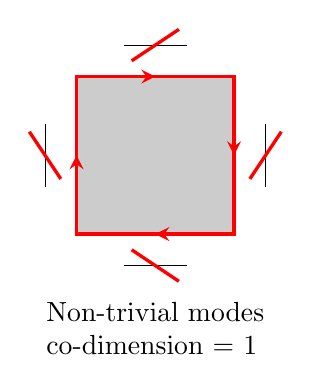
\begin{tikzpicture}
            \draw[] (-0.4,1.4) -- (0.4,1.4);
            \draw[red, very thick] (-0.3, 1.2) -- (0.3,1.6);

            \draw[] (1.4,-0.4) -- (1.4,0.4);
            \draw[red, very thick] (1.2, -0.3) -- (1.6,0.3);

            \draw[fill=black!20!white, draw=red, very thick, postaction={on each segment={mid arrow=red}}] (-1,-1) rectangle (1,1);

            \draw[] (-1.4,-0.4) -- (-1.4,0.4);
            \draw[red, very thick] (-1.2, -0.3) -- (-1.6,0.3);

            \draw[] (-0.4,-1.4) -- (0.4,-1.4);
            \draw[red, very thick] (-0.3, -1.2) -- (0.3,-1.6);
            %\draw[red, very thick, postaction={on each segment={mid arrow=red}}] (-1,-1) -- (1,-1) -- (1,1) -- (-1,1) -- cycle;
            \node[align=left] at (0, -2.2) {Non-trivial modes\\ co-dimension = 1};
        \end{tikzpicture}
        }\hspace{10mm}
        \subfigure{
        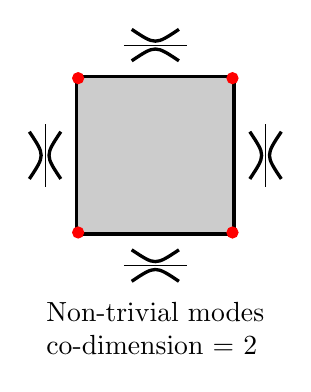
\begin{tikzpicture}
            \draw[] (-0.4,1.4) -- (0.4,1.4);
            \draw[very thick] (-0.3, 1.6) .. controls (0,1.4) .. (0.3,1.6);
            \draw[very thick] (-0.3, 1.2) .. controls (0,1.4) .. (0.3,1.2);

            \draw[] (1.4,-0.4) -- (1.4,0.4);
            \draw[very thick] (1.6, -0.3) .. controls (1.4,0) .. (1.6,0.3);
            \draw[very thick] (1.2, -0.3) .. controls (1.4,0) .. (1.2,0.3);

            \draw[fill=black!20!white, draw=black, very thick] (-1,-1) rectangle (1,1);
            \draw[fill, red] (0.98,0.98) circle (2pt) (-0.98,0.98) circle (2pt) (0.98,-0.98) circle (2pt) (-0.98,-0.98) circle (2pt) ;

            \draw[] (-1.4,-0.4) -- (-1.4,0.4);
            \draw[very thick] (-1.6, -0.3) .. controls (-1.4,0) .. (-1.6,0.3);
            \draw[very thick] (-1.2, -0.3) .. controls (-1.4,0) .. (-1.2,0.3);

            \draw[] (-0.4,-1.4) -- (0.4,-1.4);
            \draw[very thick] (-0.3, -1.6) .. controls (0,-1.4) .. (0.3,-1.6);
            \draw[very thick] (-0.3, -1.2) .. controls (0,-1.4) .. (0.3,-1.2);
            \node[align=left] at (0, -2.2) {Non-trivial modes\\ co-dimension = 2};
        \end{tikzpicture}
        }
    \end{figure}

    \blue{This definition will be refined later on.}
\end{frame}

\begin{frame}
    \frametitle{First-order topology vs second-order topology (II)} 
    \begin{figure}[]
        \centering
        \subfigure{
            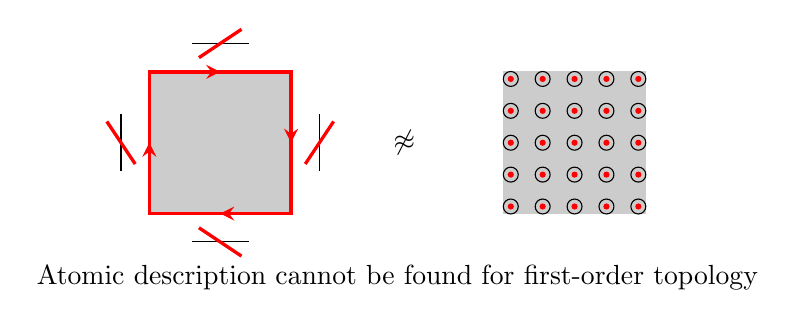
\begin{tikzpicture}[scale=0.9]
                \draw[] (-0.4,1.4) -- (0.4,1.4);
                \draw[red, very thick] (-0.3, 1.2) -- (0.3,1.6);
    
                \draw[] (1.4,-0.4) -- (1.4,0.4);
                \draw[red, very thick] (1.2, -0.3) -- (1.6,0.3);
    
                \draw[fill=black!20!white, draw=red, very thick, postaction={on each segment={mid arrow=red}}] (-1,-1) rectangle (1,1);
    
                \draw[] (-1.4,-0.4) -- (-1.4,0.4);
                \draw[red, very thick] (-1.2, -0.3) -- (-1.6,0.3);
    
                \draw[] (-0.4,-1.4) -- (0.4,-1.4);
                \draw[red, very thick] (-0.3, -1.2) -- (0.3,-1.6);
                %\draw[red, very thick, postaction={on each segment={mid arrow=red}}] (-1,-1) -- (1,-1) -- (1,1) -- (-1,1) -- cycle;
                \node[align=left] at (2.5, -1.9) {Atomic description cannot be found for first-order topology};
                \node at (2.6, 0) {$\not\approx$};

                \draw[fill,black!20!white] (4,-1) rectangle (6,1);

                \foreach \i in {0,...,4} 
                \foreach \j in {0,...,4} 
                {
                \draw[fill, red] (4.1 + 0.45*\i,-0.9 + 0.45*\j) circle (1pt);
                \draw[black] (4.1 + 0.45*\i,-0.9 + 0.45*\j) circle (3pt);
                }
            \end{tikzpicture}
            }
        \subfigure{
            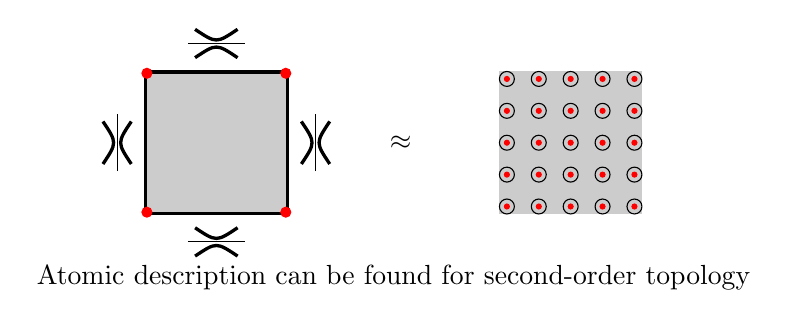
\begin{tikzpicture}[scale=0.9]
                \draw[] (-0.4,1.4) -- (0.4,1.4);
                \draw[very thick] (-0.3, 1.6) .. controls (0,1.4) .. (0.3,1.6);
                \draw[very thick] (-0.3, 1.2) .. controls (0,1.4) .. (0.3,1.2);
    
                \draw[] (1.4,-0.4) -- (1.4,0.4);
                \draw[very thick] (1.6, -0.3) .. controls (1.4,0) .. (1.6,0.3);
                \draw[very thick] (1.2, -0.3) .. controls (1.4,0) .. (1.2,0.3);
    
                \draw[fill=black!20!white, draw=black, very thick] (-1,-1) rectangle (1,1);
                \draw[fill, red] (0.98,0.98) circle (2pt) (-0.98,0.98) circle (2pt) (0.98,-0.98) circle (2pt) (-0.98,-0.98) circle (2pt) ;
    
                \draw[] (-1.4,-0.4) -- (-1.4,0.4);
                \draw[very thick] (-1.6, -0.3) .. controls (-1.4,0) .. (-1.6,0.3);
                \draw[very thick] (-1.2, -0.3) .. controls (-1.4,0) .. (-1.2,0.3);
    
                \draw[] (-0.4,-1.4) -- (0.4,-1.4);
                \draw[very thick] (-0.3, -1.6) .. controls (0,-1.4) .. (0.3,-1.6);
                \draw[very thick] (-0.3, -1.2) .. controls (0,-1.4) .. (0.3,-1.2);
                \node[align=left] at (2.5, -1.9) {Atomic description can be found for second-order topology};

                \node at (2.6, 0) {$\approx$};

                \draw[fill,black!20!white] (4,-1) rectangle (6,1);

                \foreach \i in {0,...,4} 
                \foreach \j in {0,...,4} 
                {
                \draw[fill, red] (4.1 + 0.45*\i,-0.9 + 0.45*\j) circle (1pt);
                \draw[black] (4.1 + 0.45*\i,-0.9 + 0.45*\j) circle (3pt);
                }
            \end{tikzpicture}
            }
    \end{figure}
    

\end{frame}

\begin{frame}
    \frametitle{Different kinds of atomic phases} 
    \framesubtitle{Obstructed atomic phases need crystalline symmetries to protect them.} \pause

    \only<3>{
    With $C_{4}$ atomic orbitals have to be put in on of the following Wyckoff positions relative to the center of the unit cell (corresponding to different representations of the symmetry group): 
    \begin{figure}[]
        \centering
        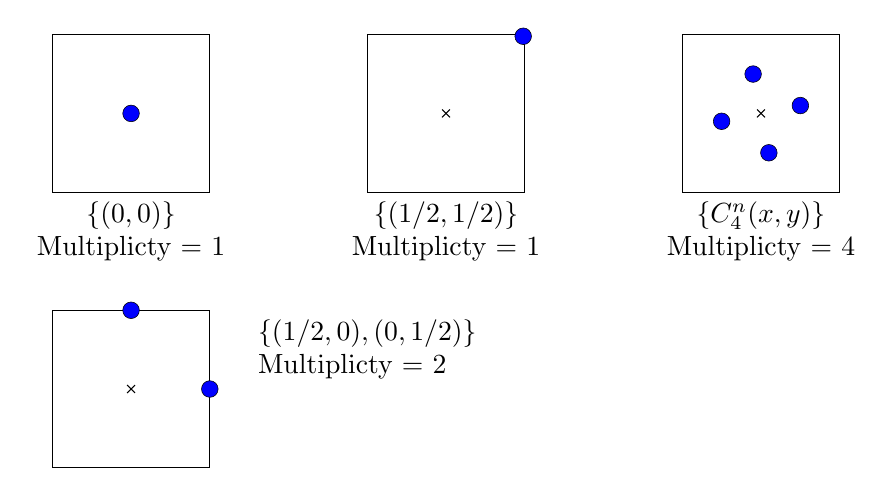
\begin{tikzpicture}
        \foreach \i in {-4,0,4} 
        {
        \draw[black] (\i,-1) rectangle (\i + 2, 1);
        }
        \draw[fill=blue, very thin] (-3,0) circle (3pt);
        \node[align=center] at (-3,-1.5) {$\{(0,0)\}$\\Multiplicty = 1};

        \draw[fill=blue, very thin] (1.98,0.98) circle (3pt);
        \draw[black] (0.95,-0.05) -- ++(0.1,0.1);
        \draw[black] (1.05,-0.05) -- ++(-0.1,0.1);
        \node[align=center] at (1,-1.5) {$\{(1/2,1/2)\}$\\Multiplicty = 1};

        \draw[fill=blue, very thin] (5.5,0.1) circle (3pt);
        \draw[fill=blue, very thin] (4.5,-0.1) circle (3pt);
        \draw[fill=blue, very thin] (4.9,0.5) circle (3pt);
        \draw[fill=blue, very thin] (5.1,-0.5) circle (3pt);
        \draw[black] (4.95,-0.05) -- ++(0.1,0.1);
        \draw[black] (5.05,-0.05) -- ++(-0.1,0.1);
        \node[align=center] at (5,-1.5) {$\{C_4^n(x,y)\}$\\Multiplicty = 4};

        \draw[black] (-4,-4.5) rectangle (-2, -2.5);
            \draw[fill=blue, very thin] (-2,-3.5) circle (3pt);
            \draw[fill=blue, very thin] (-3,-2.5) circle (3pt);
            \draw[black] (-3.05,-3.55) -- ++(0.1,0.1);
            \draw[black] (-2.95,-3.55) -- ++(-0.1,0.1);
            \node[align=left] at (0,-3) {$\{(1/2,0),(0,1/2)\}$\\Multiplicty = 2};

        \end{tikzpicture}
    \end{figure}
    }

    \only<2>{
    With $C_{2}$ atomic orbitals have to be put in on of the following Wyckoff positions relative to the center of the unit cell (corresponding to different representations of the symmetry group): 
    \begin{figure}[]
        \centering
        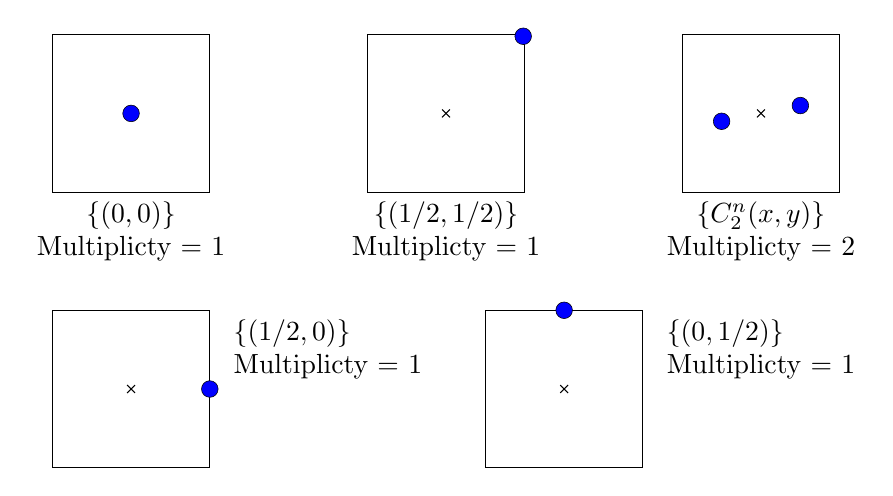
\begin{tikzpicture}
            \foreach \i in {-4,0,4} 
            {
            \draw[black] (\i,-1) rectangle (\i + 2, 1);
            }
            \draw[fill=blue, very thin] (-3,0) circle (3pt);
            \node[align=center] at (-3,-1.5) {$\{(0,0)\}$\\Multiplicty = 1};
    
            \draw[fill=blue, very thin] (1.98,0.98) circle (3pt);
            \draw[black] (0.95,-0.05) -- ++(0.1,0.1);
            \draw[black] (1.05,-0.05) -- ++(-0.1,0.1);
            \node[align=center] at (1,-1.5) {$\{(1/2,1/2)\}$\\Multiplicty = 1};
    
            \draw[fill=blue, very thin] (5.5,0.1) circle (3pt);
            \draw[fill=blue, very thin] (4.5,-0.1) circle (3pt);
            \draw[black] (4.95,-0.05) -- ++(0.1,0.1);
            \draw[black] (5.05,-0.05) -- ++(-0.1,0.1);
            \node[align=center] at (5,-1.5) {$\{C_2^n(x,y)\}$\\Multiplicty = 2};

            \draw[black] (-4,-4.5) rectangle (-2, -2.5);
            \draw[fill=blue, very thin] (-2,-3.5) circle (3pt);
            \draw[black] (-3.05,-3.55) -- ++(0.1,0.1);
            \draw[black] (-2.95,-3.55) -- ++(-0.1,0.1);
            \node[align=left] at (-0.5,-3) {$\{(1/2,0)\}$\\Multiplicty = 1};

            \draw[black] (1.5,-4.5) rectangle (3.5, -2.5);
            \draw[fill=blue, very thin] (2.5,-2.5) circle (3pt);
            \draw[black] (2.45,-3.55) -- ++(0.1,0.1);
            \draw[black] (2.55,-3.55) -- ++(-0.1,0.1);
            \node[align=left] at (5,-3) {$\{(0,1/2)\}$\\Multiplicty = 1};


            \end{tikzpicture}
    \end{figure}
    }

    \only<4>{
    With $M_x$ and $M_y$ atomic orbitals have to be put in on of the following Wyckoff positions relative to the center of the unit cell (corresponding to different representations of the symmetry group): 
    \begin{figure}[]
        \centering
        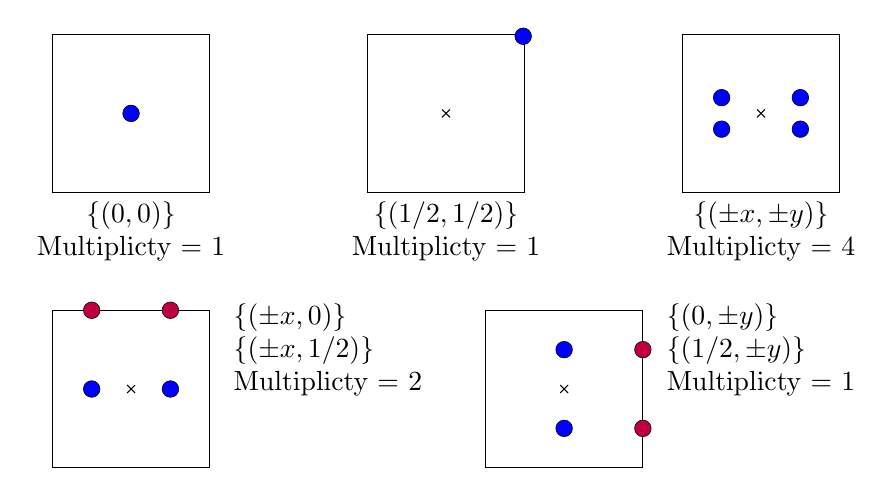
\begin{tikzpicture}
            \foreach \i in {-4,0,4} 
            {
            \draw[black] (\i,-1) rectangle (\i + 2, 1);
            }
            \draw[fill=blue, very thin] (-3,0) circle (3pt);
            \node[align=center] at (-3,-1.5) {$\{(0,0)\}$\\Multiplicty = 1};
    
            \draw[fill=blue, very thin] (1.98,0.98) circle (3pt);
            \draw[black] (0.95,-0.05) -- ++(0.1,0.1);
            \draw[black] (1.05,-0.05) -- ++(-0.1,0.1);
            \node[align=center] at (1,-1.5) {$\{(1/2,1/2)\}$\\Multiplicty = 1};
    
            \draw[fill=blue, very thin] (5.5,0.2) circle (3pt);
            \draw[fill=blue, very thin] (4.5,-0.2) circle (3pt);
            \draw[fill=blue, very thin] (4.5,0.2) circle (3pt);
            \draw[fill=blue, very thin] (5.5,-0.2) circle (3pt);
            \draw[black] (4.95,-0.05) -- ++(0.1,0.1);
            \draw[black] (5.05,-0.05) -- ++(-0.1,0.1);
            \node[align=center] at (5,-1.5) {$\{(\pm x,\pm y)\}$\\Multiplicty = 4};

            \draw[black] (-4,-4.5) rectangle (-2, -2.5);
            \draw[fill=blue, very thin] (-3.5,-3.5) circle (3pt);
            \draw[fill=blue, very thin] (-2.5,-3.5) circle (3pt);
            \draw[fill=purple, very thin] (-3.5,-2.5) circle (3pt);
            \draw[fill=purple, very thin] (-2.5,-2.5) circle (3pt);
            \draw[black] (-3.05,-3.55) -- ++(0.1,0.1);
            \draw[black] (-2.95,-3.55) -- ++(-0.1,0.1);
            \node[align=left] at (-0.5,-3) {$\{(\pm x,0)\}$\\$\{(\pm x,1/2)\}$\\Multiplicty = 2};

            \draw[black] (1.5,-4.5) rectangle (3.5, -2.5);
            \draw[fill=blue, very thin] (2.5,-3) circle (3pt);
            \draw[fill=blue, very thin] (2.5,-4) circle (3pt);
            \draw[fill=purple, very thin] (3.5,-3) circle (3pt);
            \draw[fill=purple, very thin] (3.5,-4) circle (3pt);
            \draw[black] (2.45,-3.55) -- ++(0.1,0.1);
            \draw[black] (2.55,-3.55) -- ++(-0.1,0.1);
            \node[align=left] at (5,-3) {$\{(0,\pm y)\}$\\$\{(1/2,\pm y)\}$\\Multiplicty = 1};


            \end{tikzpicture}
    \end{figure}
    }
\end{frame}


% \begin{frame}
%     \frametitle{Symmetry indicators for atomic phases.}
%     Bloch wavefunctions can be written as: 
%     \begin{align*}
%         \ket{\psi^\alpha_{\bm k}} = \sum_i e^{i\bm k \cdot \bm R_i} \ket{\phi^\alpha_{\bm R_i + \bm r_\alpha}}, && \braket{\bm r|\phi^\alpha_{\bm R_i + \bm r_\alpha}} = \phi^\alpha(\bm r - (\bm R_i + \bm r_\alpha)). 
%     \end{align*}
%     $\bm r_\alpha$ is defined relative to the the unit cell centers $R_i$. $\phi^\alpha(\bm r)$ is localized around $\bm r=0$. \pause

%     For high symmetry momenta $\bm k_*$, such that $C_n \bm k_* = \bm k_* + \bm G$, 
%     \begin{columns}
%         \begin{column}{0.6\textwidth}
%             \begin{align*}
%                 \hat C_n \ket{\psi^\alpha_{\bm k_*}} = e^{i\theta^{(n)}_\alpha} \ket{\psi^\alpha_{\bm k_*}}
%                 \end{align*}
%             The set of numbers $\{e^{i\theta^{(n)}_\alpha}\}$ at all high symmetry momenta is called the symmetry indicators. They depend on: (i) The angular momentum of the orbit $\phi^\alpha$, (ii) $r_\alpha$.
%         \end{column}
%         \begin{column}{0.4\textwidth}
%             \centering
%             \begin{tikzpicture}[scale=1.4]
%                 \draw (-1,-1) -- (1,-1) -- (1,1) -- (-1,1) -- cycle;
%                 \draw[thick,->] (-1.1,0) -- (1.4,0) node[anchor=north] {$k_x$};
%                 \draw[thick,->] (0,-1.1) -- (0,1.4) node[anchor=west] {$k_y$};
%                 \draw[fill,black] (0,0) circle (2pt) node[anchor=north east] {$(0,0)$};

%                 \draw[fill,black] (1,0) circle (2pt) node[anchor=south west] {$(0,\pi)$};
%                 \draw[fill,black] (0,1) circle (2pt) node[anchor=south east] {$(\pi,0)$};
%                 \draw[fill,black] (1,1) circle (2pt) node[anchor=west] {$(\pi,\pi)$};
%                 \end{tikzpicture}
%         \end{column}
%     \end{columns}
% \end{frame}

\begin{frame}
    \frametitle{Symmetry of Block wavefunctions}
    Bloch wavefunctions can be written as: 
    \begin{align*}
        \ket{\psi^\alpha_{\bm k}} = \sum_i e^{i\bm k \cdot \bm R_i} \ket{\phi^\alpha_{\bm R_i + \bm r_\alpha}}, && \braket{\bm r|\phi^\alpha_{\bm R_i + \bm r_\alpha}} = \phi^\alpha(\bm r - (\bm R_i + \bm r_\alpha)). 
    \end{align*}
    $\bm r_\alpha$ is defined relative to the the unit cell centers $R_i$. $\phi^\alpha(\bm r)$ is localized around $\bm r=0$. \pause
    \begin{columns}
        \begin{column}{0.6\textwidth} 
            \begin{align*}
                &\text{For $C_4$ symmetry:}\nonumber \\
                &\bm k_* = (0,0)\  \text{\&}\  (\pi,\pi) \text{\ are $C_4$ symmetric} \nonumber \\ 
                &\bm k_* = (0,\pi)\  \text{\&}\  (\pi,0) \text{\ are   $C_2$ symmetric}
            \end{align*}
            \begin{empheq}[box=\fbox]{align*}
                &\hat C_n \ket{\psi^\alpha_{\bm k_*}} = e^{i\theta_\alpha(\bm k_*)} \ket{\psi^\alpha_{\bm k_*}}
            \end{empheq}%
            $e^{i\theta_\alpha(\bm k_*)}$ at each $\bm k_*$ depend on: 

            (i) Angular momentum of $\phi^\alpha$.
            
            (ii) The position $\bm r_\alpha$.
        \end{column}
        \begin{column}{0.4\textwidth}
            \centering
            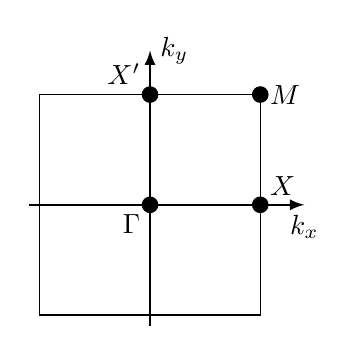
\begin{tikzpicture}[scale=1.4]
                \draw (-1,-1) -- (1,-1) -- (1,1) -- (-1,1) -- cycle;
                \draw[thick,->] (-1.1,0) -- (1.4,0) node[anchor=north] {$k_x$};
                \draw[thick,->] (0,-1.1) -- (0,1.4) node[anchor=west] {$k_y$};
                \draw[fill,black] (0,0) circle (2pt) node[anchor=north east] {$\Gamma$};

                \draw[fill,black] (1,0) circle (2pt) node[anchor=south west] {$X$};
                \draw[fill,black] (0,1) circle (2pt) node[anchor=south east] {$X^\prime$};
                \draw[fill,black] (1,1) circle (2pt) node[anchor=west] {$M$};
                \end{tikzpicture}
        \end{column}
    \end{columns}
\end{frame}

\begin{frame}
    \frametitle{Symmetry indicators as a topological invariant}
    For one or more orbitals per unit cell, the $4$ (one for each $\bm k_*$) sets $\{e^{i\theta_\alpha(\bm k_*)}\}$ are called the symmetry indicators. \pause

    Take the case with one s-orbit per unit cell:
    \begin{table}
        \centering
        \begin{tabular}{|| c | c | c ||} 
            \multicolumn{3}{ c }{\qquad \qquad \quad $\hat C_{4,2}$ eigenvalues}\\
            \hline
             $\bm k_*$ &  \quad $\bm r_\alpha = (0,0)$  \ \ & $\bm r_\alpha = (1/2,1/2)$\\ [0.5ex] 
            \hline\hline
            \  \ $\Gamma=(0,0)$ \ \   & \quad 1 \quad &  \quad 1 \quad \\ 
            \hline
            $X'=(0,\pi)$ & \quad 1 \quad &  \quad -1 \quad  \\
            \hline
            $X=(\pi,0)$ & \quad 1 \quad &  \quad -1 \quad  \\
            \hline
            $M=(\pi,\pi)$ & \quad 1 \quad &  \quad -1 \quad \\
            \hline
        \end{tabular}
    \end{table}\pause
    \begin{itemize}
        \item The different phases have different symmetry indicators. 
        \item Phases with different symmetry indicators are distinct and cannot be deformed into one another.
        \item Symmetry indicators can be used as a topological invariant. 
    \end{itemize}
\end{frame}

\begin{frame}
    \frametitle{Obstructed atomic phases and the filling anomaly}
    \begin{itemize}
        \item Corner charges can appear on these obstructed atomic phases.
        \item The key idea is that, on a sample with open boundaries, sometimes it's impossible to achieve charge neutrality while preserving the crystalline symmetry. 
    \end{itemize}\pause
    
    \begin{figure}[t]
        \centering
        \subfigure{
        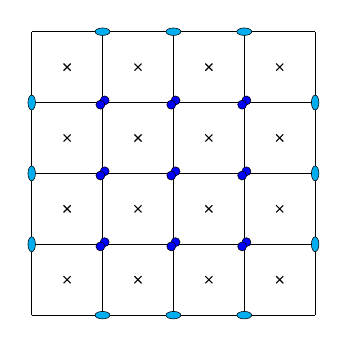
\begin{tikzpicture}[scale = 0.9]
            \draw[black] (0,0) grid(4,4);
    
            \foreach \i in {0,...,3} 
            \foreach \j in {0,...,3} 
            {
            \draw[black] (\i+0.45,\j+0.45) -- (\i+0.55,\j+0.55);
            \draw[black] (\i+0.45,\j+0.55) -- (\i+0.55,\j+0.45);
            }
    
            \foreach \i in {1,...,3} 
            \foreach \j in {1,...,3} 
            {
            \draw[fill=blue, very thin] (\i+0.03 ,\j+0.03) circle (1.8pt);
            \draw[fill=blue, very thin] (\i-0.03 ,\j-0.03) circle (1.8pt);
            
            }
    
            \foreach \i in {1,...,3} 
            {
            \draw[fill=cyan, very thin] (0 ,\i ) ellipse (1.5pt and 3pt);
            \draw[fill=cyan, very thin] (4 ,\i ) circle (1.5pt and 3pt);
            \draw[fill=cyan, very thin] (\i ,0 ) circle (3pt and 1.5pt);
            \draw[fill=cyan, very thin] (\i ,4 ) circle (3pt and 1.5pt);
            }
        \end{tikzpicture}
        }
        \subfigure{
            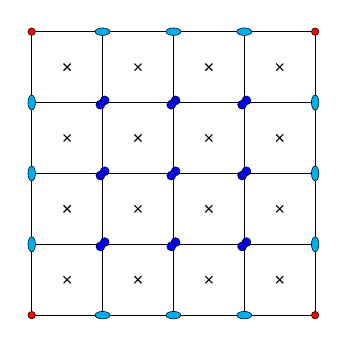
\begin{tikzpicture}[scale = 0.9]
                \draw[black] (0,0) grid(4,4);
    
                \foreach \i in {0,...,3} 
                \foreach \j in {0,...,3} 
                {
                \draw[black] (\i+0.45,\j+0.45) -- (\i+0.55,\j+0.55);
                \draw[black] (\i+0.45,\j+0.55) -- (\i+0.55,\j+0.45);
                }
        
                \foreach \i in {1,...,3} 
                \foreach \j in {1,...,3} 
                {
                \draw[fill=blue, very thin] (\i+0.03 ,\j+0.03) circle (1.8pt);
                \draw[fill=blue, very thin] (\i-0.03 ,\j-0.03) circle (1.8pt);
                }
        
                \foreach \i in {1,...,3} 
                {
                \draw[fill=cyan, very thin] (0 ,\i ) ellipse (1.5pt and 3pt);
                \draw[fill=cyan, very thin] (4 ,\i ) circle (1.5pt and 3pt);
                \draw[fill=cyan, very thin] (\i ,0 ) circle (3pt and 1.5pt);
                \draw[fill=cyan, very thin] (\i ,4 ) circle (3pt and 1.5pt);
                }
                \draw[fill=red, very thin] (0 ,0 ) circle (1.5pt);
                \draw[fill=red, very thin] (4 ,0 ) circle (1.5pt);
                \draw[fill=red, very thin] (0 ,4 ) circle (1.5pt);
                \draw[fill=red, very thin] (4 ,4 ) circle (1.5pt);
            \end{tikzpicture}
            }
            \caption*{$C_4$ symmetric lattice with two electrons per unit cell, both at the Wyckoff position $\bm r = (1/2,1/2)$. With open boundaries, both possible way of fillings give a net total charge to the system, and corner charges.}
    \end{figure}

\end{frame}

\begin{frame}
    \frametitle{Symmetry indicators as a topological invariant}
    \begin{columns}
        \begin{column}{0.55\textwidth}
            We ask with $C_4$ symmetry, and thinking of the BdG system as an insulator at half filling:
            \begin{align*}
                \mathcal{H}&(\bm k) = f_1(\bm k) \sigma_x \tau_z + f_2(\bm k) \sigma_z \tau_z  \\
                &+ \Delta g_1(\bm k) \tau_x + \Delta g_2(\bm k) \tau_y -\mu \tau_z
            \end{align*}
        \end{column}
        \begin{column}{0.45\textwidth}
            \begin{figure}[]
                \subfigure{
                    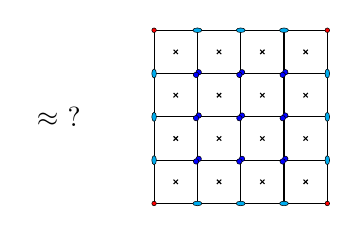
\begin{tikzpicture}[scale = 0.55]
                        \node[align=left] at (-2.2,2) {$\approx$ ?};
                        \draw[black] (0,0) grid(4,4);
            
                        \foreach \i in {0,...,3} 
                        \foreach \j in {0,...,3} 
                        {
                        \draw[black] (\i+0.45,\j+0.45) -- (\i+0.55,\j+0.55);
                        \draw[black] (\i+0.45,\j+0.55) -- (\i+0.55,\j+0.45);
                        }
                
                        \foreach \i in {1,...,3} 
                        \foreach \j in {1,...,3} 
                        {
                        \draw[fill=blue, very thin] (\i+0.03 ,\j+0.03) circle (1.8pt);
                        \draw[fill=blue, very thin] (\i-0.03 ,\j-0.03) circle (1.8pt);
                        }
                
                        \foreach \i in {1,...,3} 
                        {
                        \draw[fill=cyan, very thin] (0 ,\i ) ellipse (1.5pt and 3pt);
                        \draw[fill=cyan, very thin] (4 ,\i ) circle (1.5pt and 3pt);
                        \draw[fill=cyan, very thin] (\i ,0 ) circle (3pt and 1.5pt);
                        \draw[fill=cyan, very thin] (\i ,4 ) circle (3pt and 1.5pt);
                        }
                        \draw[fill=red, very thin] (0 ,0 ) circle (1.5pt);
                        \draw[fill=red, very thin] (4 ,0 ) circle (1.5pt);
                        \draw[fill=red, very thin] (0 ,4 ) circle (1.5pt);
                        \draw[fill=red, very thin] (4 ,4 ) circle (1.5pt);
                    \end{tikzpicture}
                    }
            \end{figure}\pause
        \end{column}
    \end{columns}
    Both have gapped bulk, gapped surfaces, and corner modes. \pause

    Need to check that there's no \emph{Wannier obstruction}:
    \begin{enumerate}
        \item Check that the Chern number is zero. \visible<5->{
\begin{tikzpicture}[scale = 0.4]
            \draw[fill,green](0,.35) -- (.25,0) -- (1,.7) -- (.25,.15) -- cycle;
            %\node[align=center, anchor = west] at (2,0.1) {Chiral symmetry};
        \end{tikzpicture}}
        \item Check the symmetry indicators if they match those of an atomic insulator. \pause
    \end{enumerate}
    \begin{framed}
        If both are satisfied, then one can deform the system to the atomic insulator it shares the symmetry indicators with.
    \end{framed}
\end{frame}

\begin{frame}
    \frametitle{Symmetry indicators as a topological invariant}
    $\[\mathcal{H}(\bm k_*), \hat C_n\] = 0 \rightarrow$ can diagonalize both. \pause

    Symmetry indicators for the $\mathcal{H}(k)$ are defined as:
    \begin{empheq}[box=\fbox]{align*}
        \hat C_n \ket{\psi^\alpha_{\bm k_*}} = \sum_i e^{i \bm R_i \cdot \bm k_*} \hat C_n \ket{u^\alpha_{\bm k_* }} = e^{i\theta_\alpha^{(n)}} \ket{\psi^\alpha_{\bm k_*}}
    \end{empheq} \pause  
    \begin{columns}
        \begin{column}{0.5\textwidth}
            \begin{table}
                \begin{adjustbox}{width=\columnwidth,center}
                    \visible<3->{
                    \begin{tabular}{|| c | c ||} 
                        \hline
                        $\bm k_*$ &  \quad $C_{4,2}$ eigenvalues of $\mathcal{H}(k_*)$  \ \ \\ [0.5ex] 
                        \hline\hline
                        \  \ $\Gamma=(0,0)$ \ \   & \quad $\{-\sgn(f_{\Gamma})\ e^{\frac{i\pi}{4}},\ \sgn(f_{\Gamma})\  e^{-\frac{i\pi}{4}}\}$ \quad \quad \\ 
                        \hline
                        $X'=(0,\pi)$ & $\{e^{\frac{i\pi}{2}}, \ e^{\frac{-i\pi}{2}}\}$  \\
                        \hline
                        $X=(\pi,0)$ & $\{e^{\frac{i\pi}{2}},\ e^{\frac{-i\pi}{2}}\} $  \\
                        \hline
                        $M=(\pi,\pi)$ & $\{-\sgn(f_{M})\ e^{\frac{i\pi}{4}}, \  \sgn(f_{M})\  e^{-\frac{i\pi}{4}}\}$ \\
                        \hline
                    \end{tabular}   }
                \end{adjustbox}
                    \vfill 
                \begin{adjustbox}{width=\columnwidth,center}
                    \visible<4->{
                    \begin{tabular}{|| c | c |c ||} 
                        \hline
                        \quad $\sgn(f_{\Gamma})$ \quad  &  \quad $\sgn(f_{M})$  \quad  
                        & \quad  \text{orbitals and Wyckoff position} \quad  \\ [0.5ex] 
                        \hline\hline
                        \  \ $+$ \ \   & \ \ $+$ \ & $j=7/2, j=5/2$ @ $\bm{r}=(0,0)$ \ \\ 
                        \hline
                        \  \ $+$ \ \   & \ \ $-$ \ & $j=7/2, j=5/2$ @ $\bm{r}=({1}/{2},{1}/{2})$ \ \\ 
                        \hline
                        \  \ $-$ \ \   & \ \ $+$ \ & $j=3/2, j=1/2$ @ $\bm{r}=({1}/{2},{1}/{2})$ \ \\ 
                        \hline
                        \  \ $-$ \ \   & \ \ $-$ \ & $j=3/2, j=1/2$ @ $\bm{r}=(0,0)$ \ \\ 
                        \hline
                    \end{tabular} }
                \end{adjustbox}   
               \end{table}
        \end{column}
        \begin{column}{0.5\textwidth}
            \visible<3->{
            $f_1(0,0) = f_2(0,0) = f_{\Gamma} $

            $f_1(\pi,\pi) = f_2(\pi,\pi) =f_{M}$
            \begin{itemize}
                \item The symmetry indicators depend on the pairing terms only indirectly.}
                \item \visible<4->{
                The condition to be in the non-trivial obstructed phase is $\sgn(f_{\Gamma}) \sgn(f_{M}) = -1$.}
            \end{itemize}
        \end{column}
    \end{columns}
    
\end{frame}

\begin{frame}
    \frametitle{Topology with $C_4$: HOTSC$_2$ with Majorana zero modes}
    The condition $\sgn(f_{\Gamma}) \sgn(f_{M}) = -1$ is guaranteed by the Dirac points in the normal state and $C_4$ symmetry. \pause
    \begin{columns} 
        \begin{column}{0.6\textwidth}
            \centering
            \begin{align*}
                &\mathcal{H}^{\text{normal}}(\bm k) = f_1(\bm k) \sigma_x + f_2(\bm k) \sigma_z \\
                &\qquad \qquad \quad =: ||f(\bm k)||\hat{\bm{n}}(\bm k)\cdot\bm{\sigma} \\
                & \hat{\bm{n}}(\bm k_* = \Gamma, M) = 1/\sqrt{2}(e_x + e_z) \\
                &\mathsf{N}_{\mathsf{w}}\left(\text{a path}\right) = \text{winding of}\ \hat{\bm n}(\bm k) \\
                &\text{Because of the the Dirac point:} \\
                &\mathsf{N}_{\mathsf{w}}\left(\gamma\circ (C_4\cdot \bar{\gamma})\right)= 1\\
                &\mathsf{N}_{\mathsf{w}}\left(\gamma\circ (C_4\cdot \bar{\gamma})\right)=2\mathsf{N}_{\mathsf{w}}(\gamma) \\
                &\mathsf{N}_{\mathsf{w}}(\gamma) = 1/2
                \end{align*}
        \end{column}
        \begin{column}{0.4\textwidth}
            \begin{figure}[]
                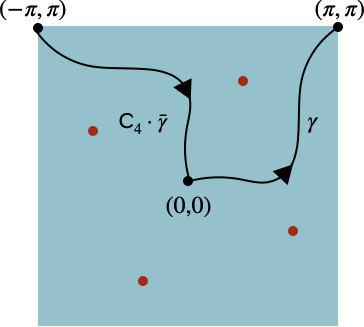
\includegraphics[scale=0.25]{C4_path.png}
            \end{figure}
        \end{column}
    \end{columns}
\end{frame}

\begin{frame}
    \frametitle{Topology with \texorpdfstring{$C_4$}{}: HOTSC$_2$ with Majorana zero modes}
    \begin{columns} 
        \begin{column}{0.55\textwidth}
            \centering
            \begin{align*}
                \mathcal{H}&(\bm k) = f_1(\bm k) \sigma_x \tau_z + f_2(\bm k) \sigma_z \tau_z\\
                &+ \Delta g_1(\bm k) \tau_x + \Delta g_2(\bm k) \tau_y-\mu \tau_z  
            \end{align*}
        \end{column}
        \begin{column}{0.45\textwidth}
            \begin{figure}[]
                \subfigure{
                    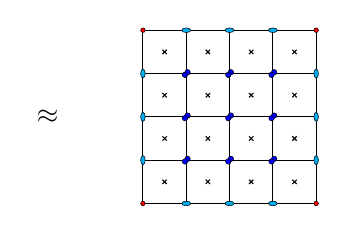
\begin{tikzpicture}[scale = 0.55]
                        \node[align=left] at (-2.2,2) {$\approx$};
                        \draw[black] (0,0) grid(4,4);
            
                        \foreach \i in {0,...,3} 
                        \foreach \j in {0,...,3} 
                        {
                        \draw[black] (\i+0.45,\j+0.45) -- (\i+0.55,\j+0.55);
                        \draw[black] (\i+0.45,\j+0.55) -- (\i+0.55,\j+0.45);
                        }
                
                        \foreach \i in {1,...,3} 
                        \foreach \j in {1,...,3} 
                        {
                        \draw[fill=blue, very thin] (\i+0.03 ,\j+0.03) circle (1.8pt);
                        \draw[fill=blue, very thin] (\i-0.03 ,\j-0.03) circle (1.8pt);
                        }
                
                        \foreach \i in {1,...,3} 
                        {
                        \draw[fill=cyan, very thin] (0 ,\i ) ellipse (1.5pt and 3pt);
                        \draw[fill=cyan, very thin] (4 ,\i ) circle (1.5pt and 3pt);
                        \draw[fill=cyan, very thin] (\i ,0 ) circle (3pt and 1.5pt);
                        \draw[fill=cyan, very thin] (\i ,4 ) circle (3pt and 1.5pt);
                        }
                        \draw[fill=red, very thin] (0 ,0 ) circle (1.5pt);
                        \draw[fill=red, very thin] (4 ,0 ) circle (1.5pt);
                        \draw[fill=red, very thin] (0 ,4 ) circle (1.5pt);
                        \draw[fill=red, very thin] (4 ,4 ) circle (1.5pt);
                    \end{tikzpicture}
                    }
            \end{figure}\pause
        \end{column}
    \end{columns}
    \begin{itemize}
        \item Corner charges are accounted for with a state localized near each corner. (Two states at each corner and you can half fill the system leading to no filling anomaly.) \pause
    \end{itemize}

    But what does it mean for our BdG system? \pause
    \begin{itemize}
        \item Particle-hole symmetry is a local symmetry $\rightarrow$ doesn't mix different corners $\rightarrow$ corner states must be Majorana zero modes. 
    \end{itemize}
\end{frame}

\begin{frame}
    \frametitle{Real space picture of the topological invariant}
    \begin{columns}
        \begin{column}{0.6\textwidth}
            The basic idea is to treat the corner of the sample as a defect, then use the Teo-Kane defect classification to detect the Majorana zero mode. 
        \end{column}
        \begin{column}{0.4\textwidth}
            \begin{figure}[]
                \centering
                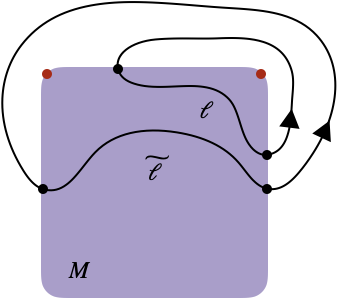
\includegraphics[scale=0.3]{Real_space_path.png}
            \end{figure}
        \end{column}
    \end{columns}
    \begin{overpic}[width=\textwidth]{defect_classification.png}
        \put (47.3,14.2) 
        {
            
\begin{tikzpicture}
                \draw[red, thick] (0,0) ellipse (5pt and 9pt);
            \end{tikzpicture}
        }
    \end{overpic}

\end{frame}

\begin{frame}
    \frametitle{Real space picture of the topological invariant}
    Model the outside by: 
    \begin{align*}
        \mathcal H_{\ms{triv}}(\bm{k})= -f_0(\sigma_x\tau_z + \sigma_z \tau_z) +\Delta \sin(k_x)\tau_x + \Delta \sin(k_y)\tau_y -\mu \tau_z
    \end{align*} \pause
    \begin{itemize}
        \item If our system with $\sgn(f_\Gamma)\sgn(f_M) = -1$ has $f_\Gamma = f_0$, then the physics of the system is completely determined by what happens near the $\Gamma$ point. 
    \end{itemize} \pause
    
    Define $\bm q$ to be a small momentum deviation from the $\Gamma$ point. The defect Hamiltonian near the $\Gamma$ point (for $\mu=0$): 
    \begin{columns}
        \begin{column}{0.6\textwidth}
            \begin{align*}
                &\mathcal H(\bm{q})=\Delta q_{x}\tau_x + \Delta q_{y}\tau_y\\ 
                &\qquad + f_0 \left[ \cos (\Phi) \sigma_x \tau_z +\sin(\Phi) \sigma_z \tau_z \right] \\ 
                &\Phi = \pi/4 \rightarrow \text{inside material} \\ 
                &\Phi = 5\pi/4 \rightarrow \text{outside material}
            \end{align*}
            
        \end{column}
        \begin{column}{0.4\textwidth}
            \begin{figure}[]
                \centering
                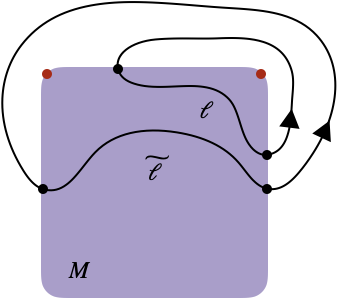
\includegraphics[scale=0.3]{Real_space_path.png}
            \end{figure}
        \end{column}
    \end{columns}

\end{frame}

\begin{frame}
    \frametitle{Real space picture of the topological invariant}
    \begin{columns}
        \begin{column}{0.6\textwidth}
            \begin{align*}
                \mathcal H(\bm{q})&=\Delta q_{x}\tau_x + \Delta q_{y}\tau_y\\ &+ f_0 \left[ \cos (\Phi) \sigma_x \tau_z +\sin(\Phi) \sigma_z \tau_z \right]
            \end{align*}
            With $C_4$ symmetry it can be shown: 
            \begin{align*}
                \mathsf{N}_{\mathsf{w}}:=\frac{1}{2\pi}\oint_{\ell} \mathrm{d}\Phi = (2n + 1).
            \end{align*}
            Adding the Chemical potential reduces the $Z$ topological invariant to a $Z_2$. 
        \end{column}
        \begin{column}{0.4\textwidth}
            \begin{figure}[]
                \centering
                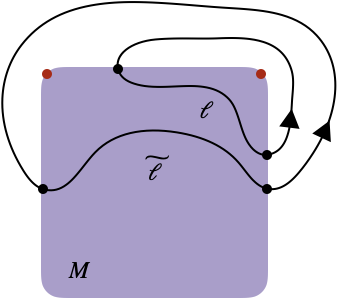
\includegraphics[scale=0.3]{Real_space_path.png}
            \end{figure}
        \end{column}
    \end{columns}

\end{frame}

\begin{frame}
    \frametitle{Summary}
    \begin{columns}
        \begin{column}{0.5\textwidth}
                \begin{table}
                    \centering
                    \def\arraystretch{0.4}
                    \begin{adjustbox}{width=\columnwidth,center}
                        \begin{tabular}{|| p{2.5cm}| p{2.5cm} | p{2.5cm}||} 
                        \hline
                        \begin{center} Model \end{center} 
                        &  \begin{center} With $C_{4}$ \end{center}   & \begin{center} With $C_{2}$  \end{center} \\ 
                        \hline\hline
                        \begin{center}
                        With PH
                        \end{center}
                        & %\rule{0pt}{4.6ex}
                        \begin{center}
                        HOTSC$_{2}$; \\
                        %\newline with 
                        corner Majorana 
                        %{\rule[-3.2ex]{0pt}{0pt}} 
                        \end{center}
                        & 
                        \begin{center}
                        BOTSC$_2$; \\
                        %\newline with 
                        corner Majorana 
                        \end{center}
                        \\ 
                        \hline
                        \begin{center}
                        Without PH
                        \end{center} &
                        \begin{center}
                        HOTI$_{2}$; \\
                        %\rule{0pt}{4.6ex}
                        % \newline with 
                        filling anomaly
                        % {\rule[-3.2ex]{0pt}{0pt}}
                        \end{center}
                        & 
                        \begin{center}
                        Trivial
                        \end{center}
                            \\ 
                        \hline
                        \end{tabular}
                \end{adjustbox}
            \end{table}
        \end{column}
        \begin{column}{0.5\textwidth}
            \begin{itemize}
                \item Today we looked at the first column of this table. 
                \item Next time we discuss the second column. 
            \end{itemize}
        \end{column}
    \end{columns}

\end{frame}
\begin{frame}
    \frametitle{A sneak peak: A cheap way of getting Majorana zero modes}
    Consider the following cheap way of getting Majorana zero modes on the corners: 
    \begin{columns}
        \begin{column}{0.4\textwidth}
            \begin{figure}[]
                \centering
                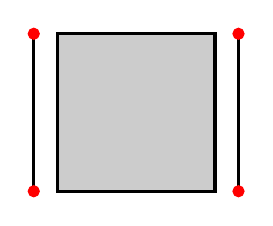
\begin{tikzpicture}
                    \draw[fill=black!20!white, draw=black, very thick] (-1,-1) rectangle (1,1);
                    \draw [black, very thick] (1.3,-1) -- (1.3,1);
                    \draw [fill,red] (1.3,-1) circle (2pt) (1.3,1) circle (2pt);
                    \draw [black, very thick] (-1.3,-1) -- (-1.3,1);
                    \draw [fill,red] (-1.3,-1) circle (2pt) (-1.3,1) circle (2pt);
                \end{tikzpicture}
            \end{figure}
        \end{column}\pause
        \begin{column}{0.6\textwidth}
            \begin{itemize}
                \item Not $C_4$ symmetric, relax $C_4$ to $C_2$.\pause
                \item Majorana zero modes can be removed without closing a bulk gap. \pause
                \item The edge gap become essential for capturing the topology of the system. 
            \end{itemize}
        \end{column}
    \end{columns}\pause
    \begin{framed}
        Such topological phases protected by an edge gap closing are called boundary obstructed topological phases.
    \end{framed}
\end{frame}



\end{document} 
 
